% Shared preamble for the English summaries in this repository.
\documentclass[11pt,a4paper]{article}
\usepackage[margin=2.2cm]{geometry}
\usepackage[T1]{fontenc}
\usepackage[utf8]{inputenc}
\usepackage{lmodern}
\usepackage{amsmath,amssymb}
\usepackage{graphicx}
\usepackage{booktabs}
\usepackage{enumitem}
\usepackage[hidelinks]{hyperref}
\setlist{itemsep=2pt,topsep=4pt}
\setlength{\parindent}{0pt}
\setlength{\parskip}{5pt}
\graphicspath{{figures/}}
\newcommand{\summaryheader}[3]{%
  \begin{center}
    {\Large\bfseries #2}\\[3pt]
    {\large #1}\\[3pt]
    {\small Arshia Goshtasbi \textbullet{} MSc Electrical Engineering (Control), Iran University of Science and Technology \textbullet{} #3}
  \end{center}
  \vspace{2pt}\hrule\vspace{8pt}
  \noindent\textit{English summary of my original Persian report, which is kept as a PDF in this folder.}\par}

\begin{document}
\summaryheader{Adaptive Control, Homework 6}{Lyapunov-based MRAC of an Unstable Plant}{Autumn 1404 (2025)}

All cases are subsystems of \texttt{HW6.slx}. They reproduce two examples from the lecture slides.

\section*{Slide 31}
The plant is $\dot x=x+3u$, which is unstable and whose parameters are unknown to the controller. The reference model is $\dot x_m=-4x_m+4r$. The controller is $u=\hat k_x x+\hat k_r r$, and both gains adapt with Lyapunov-based laws driven by the tracking error. I simulated a constant reference $r=4$ and a sinusoidal one, and plotted the output against the reference model together with $\hat k_x$ and $\hat k_r$.

\section*{Slide 34}
The same structure with an extra adapted parameter $\hat\theta$, a matched uncertainty. I plotted the output and the three estimates $\hat k_x$, $\hat k_r$ and $\hat\theta$.

\begin{center}
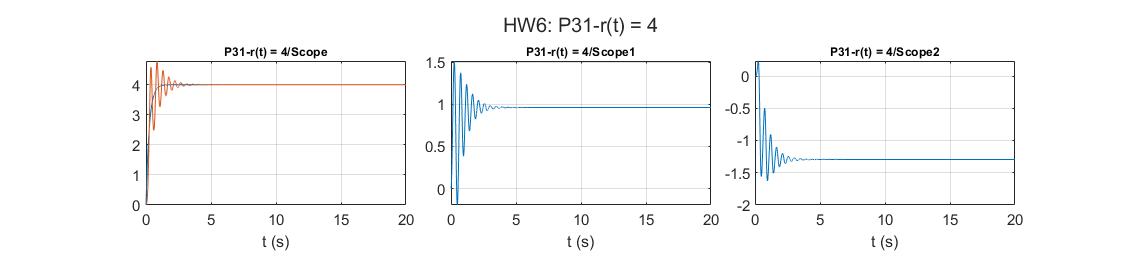
\includegraphics[width=0.9\linewidth]{P31_r_4.png}\\[2pt]
{\small Re-run in R2023b: slide 31 with $r=4$, output against the reference model, $\hat k_x$ and $\hat k_r$.}
\end{center}
\end{document}
